\markedchapter{Topological states}{Topological states of matter \& symmetries}

\blue{Sources: \cites{Akhmerov_online-course}{Asboth_topo-course}{Bernevig_topological-insulators}{Sato_superconductors}}

\blue{Topo phases occur in nature: \cite{Gehring_natural-TI}}

\red{Finish intro when chapter is more complete} %TODO

\section{Basic definitions}
{\color{blue}
\begin{itemize}
	\item Conductive properties of materials are understood in terms of band structure → Fermi energy. Conductance means Fermi level lies inside one of the bands. [picture]
	
	\item $N$-band system has hilbert space $\Hc\cong\C^N$, Hamiltonian represented by $N\times N$ matrix. Static system: $H\psi = E\psi$, eigenvalues are energy bands.
	
	\item Mostly interested in 2-band systems since only valence/conduction bands are relevant. Then $H$ is a $2\times 2$ Hermitian (for now) matrix. These are given by $H = h_0\mathbb{I} + \h\cdot\bm{\upsigma}$ in general; $h_0$ corresponds to the Fermi level and can be normalized to 0. [understand this better] → Bloch Hamiltonian [higher dimensional systems: Clifford algebra]
	
	\item For a Bloch Hamiltonian, eigenvalues are $\pm\abs{\h}$, so conductance occurs when $\h = 0$.
	
	\item Insulating Hamiltonians are adiabatically connected if they can be continuously deformed into each other without band crossings. Insulators are considered topological if they are not adiabatically connected to a reference trivial phase; then these inhabit different regions of the phase diagram → existence of edge states (not always \cite{Bernevig_topological-insulators}, footnote)
\end{itemize}
}

\subsection{Bloch theory}
{\color{blue}
\begin{itemize}
	\item We work with crystalline materials which are composed of periodically repeating unit cells.
	
	\item In the bulk, we assume the Hamiltonian is periodic in the unit cell. This enables use of Bloch's theorem \cite{Bloch_theorem} $\psi(\vb{r}) = \e^{i\k\cdot\vb{r}}u_{\k}(\vb{r})$.
	
	\item Different values of crystal momentum may yield identical eigenstates, the set of equivalence classes is the Brillouin zone
	
	\item Brillouin zone usually has $\T^n$ topology, but internal symmetries etc. may alter this \cite{Foncesca-Vaidya_nonorientable} [other sources]
\end{itemize}
}


\section{One-dimensional models}
{\color{blue}
\begin{itemize}
	\item SSH is usually introduced "physics first", but we would like to work backwards in a sense, to see how bulk topology gives rise to physical properties of a system.
\end{itemize}
}

\subsection{The Su--Schrieffer--Heeger model}
We will take the approach of deriving the Su--Schrieffer--Heeger (SSH) %TODO figure out where to introduce abbreviation
model by beginning with a generic one-dimensional crystal, and trying to make it topologically interesting the simplest way we can.

To begin with, we assume that the crystal extends infinitely in both directions. We will introduce a boundary later, but its relevant properties will turn out to be determined by the crystal's bulk topology. Concretely, we have a one-dimensional chain of unit cells indexed by $n\in\Z$; at this point, we do not make any assumptions on the internal structure of these unit cells. We require that the real-space Hamiltonian of the system is periodic in these unit cells, so that by Bloch's theorem, two crystal momenta $k$ and $k'$ are equivalent if they differ by an integer multiple of $2\pi$. This means we can take our Brillouin zone $B$ to be the interval $[-\pi,\pi]$ with the points $-\pi$ and $\pi$ identified, which is homeomorphic to $S^1$.

We might begin with a simple 2 band Bloch Hamiltonian $H(k) = \h(k)\cdot\bm{\upsigma}$, with
\[
	\h: B\cong S^1\to\R^3,\quad k\mapsto\begin{pmatrix}
		h_x(k) \\ h_y(k) \\ h_z(k)
	\end{pmatrix}.
\]
Such a Hamiltonian describes a gapped phase precisely when the map $\h$ is nowhere vanishing, so that the topological classification of these phases is given by classes of maps from $S^1$ to $\R^3$ minus the origin---that is, homotopy classes of loops in $\R^3\setminus\set{0}$. But this space has a trivial fundamental group $\pi_1\big(\R^3\setminus\set{0}\big)\cong0$, meaning all such loops can be contracted to a point; in other words, all gapped phases are adiabatically connected, and there are no topologically interesting phases.

To remedy this situation, we impose a constraint on the Hamiltonian: we require that $h_z(k)=0$, so that we effectively have a map $S^1\to\R^2$. The gapped phases are now classified by the group $\pi_1\big(\R^2\setminus\set{0}\big)\cong\Z$, indexed by winding number: loops that wind around the origin $a\in\Z$ times cannot be deformed into those with a different winding number $b\neq a$. In particular, loops with a non-zero winding number cannot be contracted to a point, and the associated phases are considered topological. Note that imposing a constraint on the Hamiltonian has made this system topologically interesting; once we move to the physical picture, we will see that this really amounts to imposing a certain symmetry on the system.

To arrive at a concrete physical system, let us begin with the simplest possible\footnote{
	Of course, our choice of $x$, $y$, and $z$ coordinates very conveniently sets us up to arrive at the SSH model. However, mathematically speaking, all similar models are related by a simple change of basis.}
distinct states, one trivial and one topologically interesting:
\[
	\h_{\rm triv}(k) = \begin{pmatrix}
		1 \\ 0 \\ 0
	\end{pmatrix},\qquad \h_{\rm top}(k) = \begin{pmatrix}
		\cos(k) \\ \sin(k) \\ 0
	\end{pmatrix}.
\]
To characterise a phase transition between these two states, we look at the linear combination $\h(k) = v\h_{\rm triv}(k) + w\h_{\rm top}(k)$, with $v,w\geq0$. The phase described by the resulting Bloch Hamiltonian is trivial when $v>w$, gapless (i.e.\ conducting) when $v=w$, and topological when $v<w$; see Figure \ref{fig:phases}.
\begin{figure}[htb!]
	\centering
	\begin{subfigure}{.3\textwidth}
		\centering
		\begin{tikzpicture}
			\begin{axis}[
				axis equal image,
				axis lines=middle,
				axis line style={->},
				xtick={-1,1}, ytick={-1,1},
				xmin=-1.2, xmax=1.2,
				ymin=-1.2, ymax=1.2,
				xlabel=$h_x$, ylabel=$h_y$,
				width=6.5cm,
				]
				\addplot+[mark options={black}] coordinates {(0,0)};
				\addplot [
				samples=100, domain=0:2*pi, color=teal, thick,
				] ( {.3*cos(deg(x)) + .5}, {.3*sin(deg(x))} );
			\end{axis}
		\end{tikzpicture}
		\caption{$v=0.5$, $w=0.3$}
	\end{subfigure}
	\hfil
	\begin{subfigure}{.3\textwidth}
		\centering
		\begin{tikzpicture}
			\begin{axis}[
				axis equal image,
				axis lines=middle,
				axis line style={->},
				xtick={-1,1}, ytick={-1,1},
				xmin=-1.2, xmax=1.2,
				ymin=-1.2, ymax=1.2,
				xlabel=$h_x$, ylabel=$h_y$,
				width=6.5cm,
				]
				\addplot+[mark options={black}] coordinates {(0,0)};
				\addplot [
				samples=100, domain=0:2*pi, color=teal, thick,
				] ( {.4*cos(deg(x)) + 0.4}, {.4*sin(deg(x))} );
			\end{axis}
	\end{tikzpicture}
	\caption{$v=w=0.4$}
	\end{subfigure}
	\hfil
	\begin{subfigure}{.3\textwidth}
		\centering
		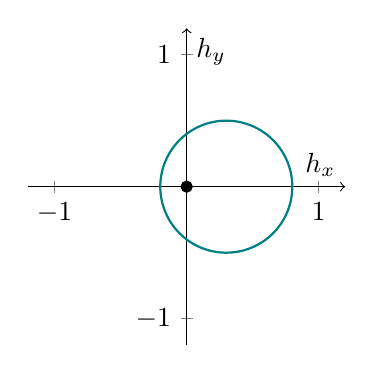
\begin{tikzpicture}
			\begin{axis}[
				axis equal image,
				axis lines=middle,
				axis line style={->},
				xtick={-1,1}, ytick={-1,1},
				xmin=-1.2, xmax=1.2,
				ymin=-1.2, ymax=1.2,
				xlabel=$h_x$, ylabel=$h_y$,
				width=6.5cm,
				]
				\addplot+[mark options={black}] coordinates {(0,0)};
				\addplot [
				samples=100, domain=0:2*pi, color=teal, thick,
				] ( {.5*cos(deg(x)) + 0.3}, {.5*sin(deg(x))} );
			\end{axis}
		\end{tikzpicture}
		\caption{$v=0.3$, $w=0.5$}
	\end{subfigure}
	\caption{Contours in Hamiltonian space for (a) trivial, (b) conducting and (c) topological phases.}
	\label{fig:phases}
\end{figure}

Now that we have a simple setup, it's time to analyse the physics. Concretely, the momentum space Hamiltonian is given by
\begin{align*}
	H(k) &= \h(k)\cdot\bm{\upsigma} = \big(v + w\cos(k)\big)\sigma_x + w\sin(k)\sigma_y = \begin{pmatrix}
		0 & v + w\e^{-ik} \\
		v + w\e^{ik} & 0
	\end{pmatrix}.
\end{align*}
We can set up a Fourier transform to real space by rewriting this suggestively in terms of the unit cell index $n$:
\[
	H(k) = \e^{-ik(n-n)}\begin{pmatrix}
		0 & v \\
		v & 0
	\end{pmatrix} + \e^{-ik\big((n+1)-n\big)}\begin{pmatrix}
		0 & w \\
		0 & 0
	\end{pmatrix} + \e^{-ik\big(n-(n+1)\big)}\begin{pmatrix}
		0 & 0 \\
		w & 0
	\end{pmatrix}
\]
{\color{red} I need to work out the details of this Fourier transform later, my calculations aren't working out. Transforming from a periodic Brillouin zone to (discrete or infinite) real space is breaking my brain. I imagine it needs to look something like this (where $M_{0/\pm1}$ are the three matrices above):
\begin{align*}
	\hat{H} &= \int_B H(k) \ket{k}\bra{k} \\
		&= \int_{-\pi}^{\pi}\frac{\dd{k}}{2\pi} \left(\sum_{a\in\{0,\pm1\}}\e^{-ika}M_a\right) \left(\sum_{n}\e^{-ikn}\ket{n}\right) \left(\sum_{n'}\bra{n'}\e^{ikn'}\right) \\
		&= \sum_{a,n,n'}\left(\int_{-\pi}^{\pi}\frac{\dd{k}}{2\pi}\e^{-ik(a+n-n')}\right)M_a\ket{n}\bra{n'} \\
		&= \sum_{a,n,n'}\delta_{n+a,n'}M_a\ket{n}\bra{n'} \\
		&= \sum_{a,n}M_a\ket{n}\bra{n+a}
\end{align*}
But I don't fully understand the first step, the sign of $a$ is wrong and normalization is broken. Maybe it's easier to discretize first and do a DFT?}

{\color{blue}
\begin{itemize}
	\item It follows [how exactly?] that we can write the Hamiltonian in a unit cell basis as
	\[
		\hat{H} = \sum_{n=-\infty}^{\infty}\left[\ket{n}\bra{n}\otimes\begin{pmatrix}
			0 & v \\
			v & 0
		\end{pmatrix} + \left(\ket{n+1}\bra{n}\otimes\begin{pmatrix}
			0 & w \\
			0 & 0
		\end{pmatrix} + {\rm h.c.}\right)\right]
	\]
	
	\item Mention tight binding somewhere around this point
\end{itemize}
}

It's clear that we have a term parametrized by $v$ which acts within the unit cells, and terms depending on $w$ which act between neighbouring unit cells. To further elucidate the structure of these interactions, we go to a finite chain of length $N$; the Hamiltonian then becomes
\[
	\hat{H} = \sum_{n=0}^{N}\ket{n}\bra{n}\otimes\begin{pmatrix}
		0 & v \\
		v & 0
	\end{pmatrix} + \sum_{n=0}^{N-1}\left(\ket{n+1}\bra{n}\otimes\begin{pmatrix}
		0 & w \\
		0 & 0
	\end{pmatrix} + {\rm h.c.}\right),
\]
where we've introduced open boundary conditions on the ends of the chain, allowing us to study the boundary behaviour in a moment. We can then expand the tensor product in order to cast the Hamiltonian into a full $2N\times 2N$ matrix:
\[
	\hat{H} = \begin{pNiceMatrix}
		\Block[borders={bottom,right,tikz=dashed}]{2-2}{}
					 0 & v & \Block[borders={bottom,right,tikz=dashed}]{2-2}{}
							 0 & 0 & \Block{4-4}{0} &        &   & \\
					 v & 0 & w & 0 &                &        &   & \\
		\Block[borders={bottom,right,tikz=dashed}]{2-2}{}
					 0 & w & 0 & v &                &        &   & \\
					 0 & 0 & v & 0 &                &        &   & \\
		\Block{4-4}{0} &   &   &   &                & \Ddots & 0 & 0 \\
					   &   &   &   & \Ddots         &        & w & 0 \\
					   &   &   &   &              0 & w      & 0 & v \\
					   &   &   &   &              0 & 0      & v & 0
	\end{pNiceMatrix}.
\]
A clear interpretation of this system presents itself to us immediately: it describes a chain of $2N$ sites, with alternating hopping amplitudes $v$ and $w$ between neighbouring sites. The unit cells now consist of two of these sites, and $v$ and $w$ are referred to as the \emph{intra-cell} and \emph{inter-cell} hoppings, respectively. In particular, the gapless phase $v=w$ corresponds to a chain where all hoppings are equal; intuitively, this allows electrons to move around freely along the chain, whereas they are confined around the stronger hoppings in the insulating cases.

The division of our unit cells into two sites allows us to distinguish two \emph{sublattices} of the crystal, which we label $A$ and $B$. We then simplify our notation by labelling quantum states according to the sublattice that they are localized to:
\[
	\ket{n,A} \equiv \ket{n}\otimes\begin{pmatrix}
		1 \\ 0
	\end{pmatrix},\quad \ket{n,B} \equiv \ket{n}\otimes\begin{pmatrix}
		0 \\ 1
	\end{pmatrix}.
\]
In this notation, our Hamiltonian becomes
\begin{equation}\label{eq:ssh-sublattice}
	\hat{H} = \left(\sum_{n=0}^{N}v\ket{n,B}\bra{n,A} + \sum_{n=0}^{N-1}w\ket{n+1,A}\bra{n,B}\right) + {\rm h.c.}
\end{equation}

The picture of alternating hoppings that we have arrived at is precisely the original motivation for this model: it was first introduced in 1979 by Wu-Pei Su, John Robert Schrieffer, and Alan J. Heeger in order to study the properties of polyacetylene (Figure \ref{fig:polyacetylene}), a polymer chain which features alternating single and double covalent bonds \cites{SSH_model}{SSH_model2}.
\begin{figure}[htb!]
	\centering
	\includegraphics[width=.8\linewidth]{Images/polyacetylene} %TODO svg
	\caption{Structural diagram of polyacetylene. Electrons are transported more readily along the double bonds, which is modelled using a larger hopping potential.}
	\label{fig:polyacetylene}
\end{figure}
This material displays unexpectedly high conductivity when doped with halogen impurities, and the SSH model helps explain this behaviour.

To understand how this conductive behaviour comes about, we need to examine the differences between the trivial and the conductive phase somewhat more closely. At a first glance, the two phases appear to be identical: if we choose the unit cell in polyacetylene in such a way that the stronger double bond represents the intra-cell hopping $v$, then we are in the trivial phase $v>w$, and if we center the unit cell around a single bond, we have $v<w$ and the phase is topological. In either case we expect valence electrons to remain localized around the double bonds, leading to the same insulating bulk behaviour.\footnote{
	The attentive reader might wonder why the conductive $v=w$ phase does not occur naturally in this system. This is a result of the so-called Peierls transition: in a nutshell, introducing a band gap locally lowers the energy of the (filled) valence band and raises that of the (empty) conduction band. This makes it energetically favourable for atoms in the chain to pair up, in a process referred to as dimerisation.}

The difference between the two phases only becomes apparent when we look at the endpoints of the chain. For example, the leftmost atom is not subject to any inter-cell hopping, and it is only connected to the other atom in its unit cell. In the trivial case this connection is strong and the two atoms share their valence electrons. On the other hand, in the topological phase the second atom from the left prefers to share electrons with its right-hand neighbour, and the leftmost atom becomes isolated. In the limit where $v$ goes to zero, this isolation becomes complete and the edge sites carry zero-energy eigenstates: in this case only the second term in the Hamiltonian (\ref{eq:ssh-sublattice}) survives, and we have
\begin{align*}
	\hat{H}\ket{1,A} = \hat{H}\ket{N,B} = 0.
\end{align*}
Even for non-zero $v$ the topological phase has edge modes, which can be shown to become highly localized and approach zero energy in the $N\to\infty$ limit. The exact mechanics of this are beyond the scope of this review; the interested reader is referred to e.g.\ \cite{Asboth_topo-course}. The salient point is that the boundary modes of the chain are gapless: their energy eigenvalues have a degeneracy at the Fermi level $\varepsilon_F = 0$.
%TODO picture?

Something remarkable has happened: we have started from a topological description of a gapped bulk phase, and the resulting physical effects appear as gapless edge modes on the boundary of the material. As we will see, this is a fairly\footnote{
	This is not a completely general statement: topological phases with gapped edge modes have been shown to be theoretically feasible \cite{Freedman_gapped-edge}. For our purposes, it will do to restrict our attention to the gapless edge modes.}
general feature of topological phases of matter, called the \emph{bulk-boundary correspondence}. We can think of it as being a result of the inability to go continuously from a topological gapped phase to a trivial one in real space; in particular, the outside boundary of an idealised material connects to the vacuum, which is also considered a trivial gapped phase.

{\color{blue}
\begin{itemize}
	\item Discuss physics of polyacetylene (solitons on trivial/topological interface) and experimental observations of solitons + berry phase \cites{Meier_SSH-soliton}{Atala_SSH-Zak}
	
	\item We can now physically interpret the meaning of setting $h_z = 0$: it ensures that hopping only occurs between the two sublattices $A$ and $B$, and not within them (i.e.\ there are only off-diagonal elements in the internal degrees of freedom). If we define the sublattice projection operators
	\[
		\hat{P}_A = \mathbb{I} \otimes \begin{pmatrix}
			1 & 0 \\ 0 & 0
		\end{pmatrix},\quad \hat{P}_B = \mathbb{I} \otimes \begin{pmatrix}
			0 & 0 \\ 0 & 1
		\end{pmatrix}
	\]
	then the Hamiltonian obeys
	\[
		\hat{P}_A\hat{H}\hat{P}_A = \hat{P}_B\hat{H}\hat{P}_B = 0
	\]
	and so since $\hat{P}_A + \hat{P}_B$ is the identity we have
	\begin{align*}
		\hat{H} &= (\hat{P}_A + \hat{P}_B)\hat{H}(\hat{P}_A + \hat{P}_B) \\
			&= \hat{P}_A\hat{H}\hat{P}_B + \hat{P}_B\hat{H}\hat{P}_A \\
			&= (\hat{P}_A - \hat{P}_B)\hat{H}(\hat{P}_B - \hat{P}_A) \\
			&\equiv -\hat{\Gamma}\hat{H}\hat{\Gamma}
	\end{align*}
	with $\hat{\Gamma}\equiv\hat{P}_A - \hat{P}_B$ having the property that $\hat{\Gamma} = \hat{\Gamma}^{-1} = \hat{\Gamma}\dagger$; this is called sublattice symmetry and it also applies to the momentum space Hamiltonian $H(k)$.
	
	\item An immediate consequence of our setup is that the trivial and topological phase become adiabatically connected if we allow for sublattice symmetry breaking ($h_z \neq 0$).
	
	\item Talk more about $\Z$ invariant (next nearest neighbour hopping etc.)
\end{itemize}
}

\subsection{The Kitaev chain}

{\color{blue}
\begin{itemize}
	\item Introduce Majorana modes
	
	\item Talk about superconductivity
	
	\item Discuss $\Z_2$ invariant vs.\ $\Z$ for SSH topologically
\end{itemize}
}


\section{Two-dimensional models}

\subsection{Quantum Hall effect}

\subsection{The Kane--Mele model}


\markedsection{Symmetry classes}{Classification of symmetries}